
\documentclass[10pt,letterpaper]{article}
\usepackage[top=0.85in,left=0.85in,footskip=0.75in]{geometry}
% amsmath and amssymb packages, useful for mathematical formulas and symbols
\usepackage{amsmath,amssymb}
% Use adjustwidth environment to exceed column width (see example table in text)
\usepackage{changepage}
% Use Unicode characters when possible
\usepackage[utf8x]{inputenc}
% textcomp package and marvosym package for additional characters
\usepackage{textcomp,marvosym}
% cite package, to clean up citations in the main text. Do not remove.
\usepackage{cite}
\usepackage{url}
% Use nameref to cite supporting information files (see Supporting Information section for more info)
%\usepackage{nameref,hyperref}
% line numbers
%\usepackage[right]{lineno}

%\usepackage{natbib}
\usepackage{graphicx}
\usepackage{float}

% color can be used to apply background shading to table cells only
\usepackage[table]{xcolor}

% array package and thick rules for tables
\usepackage{array}
\usepackage{dsfont}

\usepackage{todonotes}
\usepackage{comment}

% referencing supplement-material
\usepackage{xr}
\externaldocument{./supplement}
%\usepackage{cleveref}



%% END MACROS SECTION

\title{Triqler for Protein Summarization of Data from Data Independent Aquisition Mass Spectrometry}
\author{Patrick Truong \and Matthew The \and Lukas K\"{a}ll}


\begin{document}
%\linenumbers
\maketitle

%Here I want to reference a figure that is in my supplementary content \cref{supp-fig:model_selection_criteria}.

%Here is a ref to the supplement, we have a Supplementary Figure \ref{fig:diff_vs_hela_find_a_better_label}.

\begin{abstract}

A frequent desired goal when processing data from quantative shotgun proteomics experimentsis a list of proteins that are differentially abundant under the examined experimentak conditions. Unfortunatly, this is a challenging process, as the mass spectrometer analyses the proteolytic peptides of a protein and not the proteins themselves. We have previously designed a Bayesian hirarchical probabilistic model, Triqler, for combining peptide identification and quantification errors into probabilities of proteins being differentially abundant. 

Here we show that Triqler, is well compatible with data-independent acquisition data, despite being designed for data-dependent acquisition data. Furthermore, we find that it has better performance than other protein summarization tools, when comparing against a set of state of the art DIA processing methods. 
\end{abstract}
  

\section*{Introduction}

Label-free quantification (LFQ) using Mass spectrometry (MS)-based proteomics enables efficient determination of differential concentrations of proteins in complex mixtures. The processing of data from such experiments requires multiple different steps, all subjects to errors. 
For the analysis of mass spectrometry-based proteomics data, just as any other type of analysis of complex data, the individual computational methods for all the steps in the processing affect the final results. It is therefore quite hard to evaluate the influence of the individual tools, which should not stop the field from trying to establish the features of the different processing steps and how they influence end-results \cite{dufresne2014abrf,gatto2016testing,navarro2016multicenter}. Unbiased comparisons of software tools are challenging for several reasons \cite{dufresne2014abrf}. Methods can be assessed by scientist lacking relevant expertise, the tested methods may be lacking sufficient documentation and the interpretation of test results may be subjective \cite{yates2012toward} \cite{leprevost2014best} \cite{pak2013clustering} \cite{faircomparison2015}. By using the same data set we can assure that the data set is processed consistently and further the analysis by extending it to protein summarization procedures.


We have previously designed a hierarchical Bayesian model, Triqler, able to control for errors from both the identification and quantification process in such experiments\cite{The2018Integrated}. By integrating the errors probabilities from identification and quantification one can obtain better accuracy in calling differentially abundant proteins \cite{The2018Integrated}.   Triqler was designed for handling LFQ data from Data-dependent acquisition (DDA). However, many labs prefer Data-independent acquisition (DIA) mass spectrometry \cite{venable2004automated} as they find that it gives more reproducible peptide detection, and allow for a broader dynamical range in quantification \cite{bern2010deconvolution,zhang2020DIA}, compared to DDA. 

Here, we set out to investigate Triqler ability to summarize protein concentrations from peptide abundances derived from DIA data. We primarily used the LFQBench from Navarro et al. \cite{navarro2016multicenter} for the evaluation. In the original benchmark, Navarro et al. included a comparison of different protein summarization strategies and found that the so-called Top3 method generally resulted in lower variance and better quantification accuracy than the built-in methods from the tested methods\cite{navarro2016multicenter}. However, there are reasons to believe that more sophisticated methods would yield better protein quantification than the Top3-method. Simple summarization methods based on mean and median peptide intensity has been shown to produce unreliable protein abundance estimates \cite{goeminne2015summarization}, and more advanced summarization strategies for LFQ data has been proposed in literature \cite{silva2006absolute,cox2014accurate}, and summarization techniques such as PQPQ~\cite{forshed2011enhanced}, msStats~\cite{choi2014msstats}, Diffacto~\cite{zhang2017covariation}, MSqRob2~\cite{sticker2020robust} and Triqler~\cite{The2018Integrated} has all been shown to outperform Top3 and there currently exists no reason why said methods would not theoretically be able to perform well for DIA data. Hence, we found it apt to benchmark Triqler against a set of state-of-the-art protein summarization methods using peptide quantities from the LFQBench DIA data set.
 
 
\section*{Materials and methods}


\subsection*{Data description}
\subsubsection*{Mass spectrometry data}


We downloaded the LFQBench dataset~\cite{navarro2016multicenter} from PRIDE identifier PXD002952. Here we used the TripleTOF6600 section of the study, which was harvested with a setup of 32 fixed windows ms2-windows. We also restricted ourselves to the low ratio difference samples, referred to as the HYE124 hybrid proteome samples in the original study. That consists of triplicates of Sample A composed of tryptically digested proteins from 65\% w/w HeLa, 30\% w/w yeast, and 5\% w/w \textit{E. coli} cells, and triplicates of Sample B, composed of 65\% w/w, 15\% w/w yeast, and 20\% w/w \textit{E. coli} proteins. Samples from HYE110 and the TripleTOF5600 section of HYE124 were omitted in this study. Further details about mass spectrometric instrumentation and data acquisition are available in Navarro et al.~\cite{navarro2016multicenter}. The \verb|.wiff| files were converted to \verb|.mzML| files in a centroided format using msconvert (using windows OS msconvert version 3.0) with peakPicking filter msLevel=1-). 


\subsubsection*{Sequence database}

Uniprot FASTA files with one protein sequence per gene were downloaded for each species (UP000005640, UP000000625, and UP000002311, acquired on 2021-06-16). The unfiltered FASTA files contained 20 590 human proteins, 6 046 yeast proteins, and 4 373 \textit{E. coli} proteins. To reduce the effect of the different protein inference strategies for the tested protein summarization tools, a modified .fasta file, without shared peptides, was used for database search. The filter randomly removed protein sequences with shared peptides, so that the final database did not contain any tryptic peptides with length $>$7 amino acids mapping to peptides shared with other proteins. After filtering the FASTA file contained 20 302 proteins (288 human proteins fewer proteins than an unfiltered database), 5 848 yeast proteins (198 yeast proteins fewer proteins than an unfiltered database), and 4 306 \textit{E. Coli} proteins (67 \textit{E. Coli} proteins than unfiltered database). Replacing the I/L amino acids to handle mass-equivalence did not result in any considerable differences (See Supplementary Table \ref{table:proteins_in_database}). We also added pseudo-reverse sequences to the database as decoys for target-decoy analysis using OpenSwathDecoyGenerator. 


\subsection*{General workflow}

We used two separate strategies to generate peptide abundances from the DIA-runs, first we used a spectral library consisting of selected spectra from separate DDA runs, we refer to this workflow as ID hereon, and secondly, we searched pseudo-spectra generated directly from the DIA data, we will refer to this workflow as PS from hereon. The workflows are shown in figure \ref{fig:flowchart}. We will describe the parameter choices of both these two methods below.

\begin{figure}[htp]
    \centering
    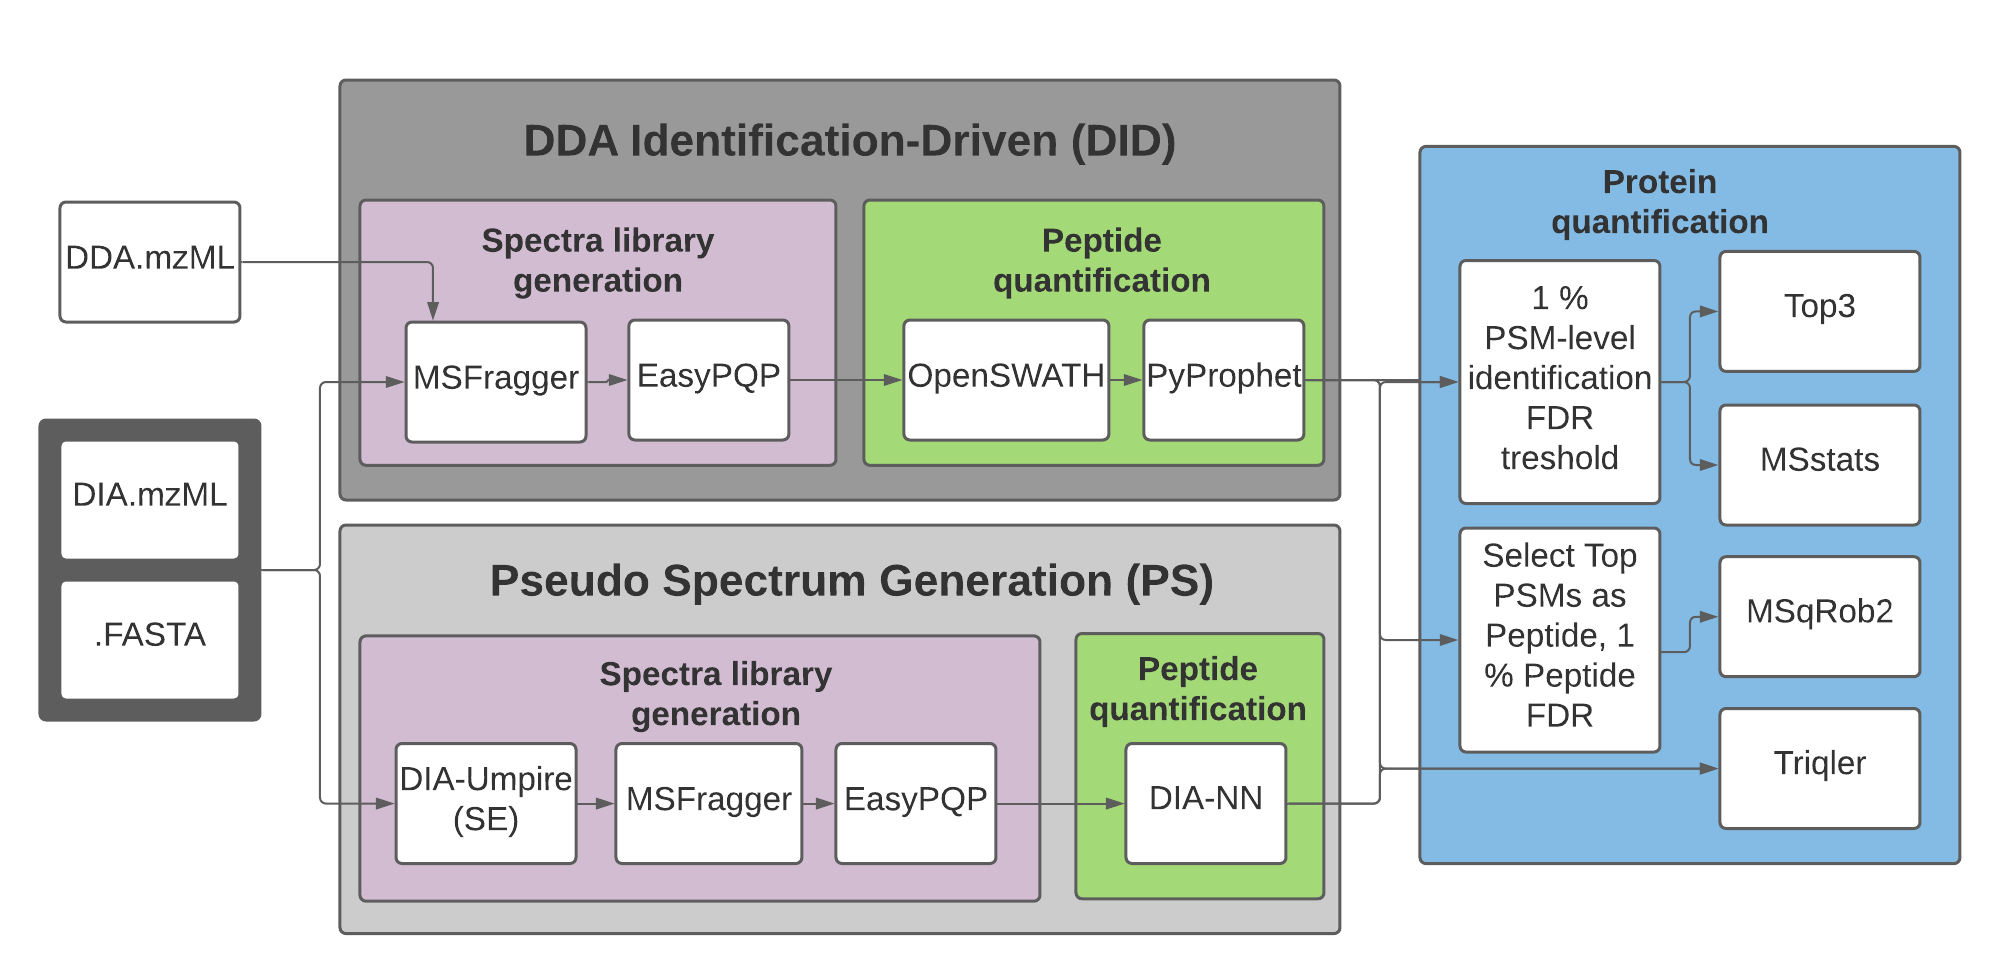
\includegraphics[width=1.0\linewidth]{../../result/report_plots/DIA_benchmark_truncated.png} 
    \caption{{\bf The DDA identification-driven matching (ID) and pseudo spectrum workflow pipelines (PS).} In the pipelines DIA-Umpire(SE), MSFragger and EasyPQP is run from Fragpipe (\protect\url{https://fragpipe.nesvilab.org/}). Threshhold at 1\% PSM-level or peptide-level identification FDR or no filtration was used for filtering before protein summarization depending on the requirements of the summarization tools. \label{fig:flowchart}}      
\end{figure}



\subsubsection*{DDA identification-driven (ID) spectral library}

For the ID workflow we searched the LFQBench provided DDA runs with MSFragger\cite{kong2017msfragger} with default settings (Precursor mass tolerance of [-20, 20] ppms, fragment tolerance of 20 ppms, Calibration and Optimization: "Max calibration, parameter optimization", isotope error: 0/1, Data type: DDA, Load rules: stricttrypsin, Cut after: KR, Cleavages: ENZYMATIC, Missed cleavages: 2, Clip N-term M: True, Peptide length of [7, 50], Peptide mass range of [500, 5000], Split database: 1, and allowing for oxidation on methionine and protein N-terminus modifier as variable modifications), and constructed a spectral library with EasyPQP \cite{easypqp} to from the DDA-search results with default setting (RT Calibration: "Automatic selection of a run as reference RT", RT Lowess Fraction: 0.1, UniMod annotation tol(Da), Fragment annotation tol(ppm): 15, and the default PSM-level threshold of 0.01, peptide-level FDR of 0.01, and protein-level FDR of 0.01). Decoys for the spectral library were generated with OpenSwathDecoyGenerator with a pseudo-reverse method. The spectral library was subsequently matched to the DIA data with the OpenSwath Workflow and PyProphet\cite{teleman2015diana} was used for computing false discovery rate (m\_score) for the peptide identification. This resulted in a set of detected peptides together with their assessed peptide identification accuracies and abundance estimates (Supplementary Table \ref{fig:osw_peptide_and_protein_id} shows the number of identified peptides and proteins).


\subsubsection*{Pseudo Spectra generation (PS) spectral library}

For the PS workflow we also used the fragpipe software, employing DIA-Umpire to extract pseudo-spectra from the DIA data. The DIA-Umpire parameters was set to default values (MS1 PPM: 10, MS2 PPM: 20, Max Missed Scans: 1, Mass Defect Filter: True, RP max: 25, RF max: 500, Corr Treshold: 0, Delta Apex: 0.2, RT Overlap 0.3, Mass Defect Offset 0.1, Isotope Pattern: 0.3, MS1 SN: 1.1, MS2 SN: 1.1, Adjust Fragment Intensity: True). The pseudo-spectra were subsequently searched using using MSFragger with default settings (Precursor mass tolerance of [-20, 20] ppms, fragment tolerance of 20 ppms, Calibration and Optimization: "Max calibration, parameter optimization", isotope error: 0/1, Data type: DDA, Load rules: stricttrypsin, Cut after: KR, Cleavages: ENZYMATIC, Missed cleavages: 2, Clip N-term M: True, Peptide length of [7, 50], Peptide mass range of [500, 5000], Split database: 1, and allowing for oxidation on methionine and protein N-terminus modifier as variable modifications). A spectral library was build from the resulting PSMs using easyPQP with default setting (RT Calibration: ``Automatic selection of a run as reference RT'', RT Lowess Fraction: 0.1, UniMod annotation tol(Da), Fragment annotation tol(ppm): 15, and the default PSM-level treshold of 0.01, peptide-level FDR of 0.01, and protein-level FDR of 0.01). DIA-NN was used for peptide quantifications with settings specified in \url{https://fragpipe.nesvilab.org/docs/tutorial_DIA.html#quantify-with-dia-nn} (Protein inference: ``Off'', Quantification strategy: ``Robust LC (High accuracy)'', Precursor FDR (\%): 1.0, Protease: ``Trypsin/P'', Missed cleavages: 1, Maximum number of cariable modifications: 0, N-term M excision: True, C carbamidomethylation: True, Peptide length: [7, 30], Precursor m/z range: [300, 1800], Fragment ion m/z range: [200, 1800], Mass accuracy: 0.0, MS1 accuracy: 0.0, Scan window: 0, Use isotopologues: True, Remove likely interferences: True, Neural network classifier: ``Single-pass mode'', Protein inference: Genes, Cross-run normalization: ``RT-dependent'', Library generation: ``Smart profiling''). Too compute false discover rates DIA-NN uses a built-in custom implementation of the mProphet algorithm to compute $q$~values \cite{reiter2011mprophet, demichev2020dia} (Supplementary Table \ref{fig:diann_peptide_and_protein_id} shows the number of identified peptides and proteins). 
 
\subsection*{Protein summarization}

The peptide quantities were summarized to proteins using the average of the three most intense peptides (We call it Top3), MSstats, MSqRob2, and Triqler for both the ID spectral library and the PS spectra library pipelines. 

\subsubsection*{Top3}

We implemented a short script that for each protein selected the average of the 3 most abundant PSMs for each protein and sample. In samples only having two PSMs available these were also included, still represented by their average, however, proteins with one or zero PSMs per sample were excluded. PSMs were filtered at an 1\% FDR before performing the Top3 protein summarization. 

\subsubsection*{MsStats}

We installed MSstats version 3.18.5 using R/Bioconductor (available at \url{https://www.bioconductor.org/packages/release/bioc/html/MSstats.html}). MSstats use feature-level data, allowing for multiple PSM hits per peptide identification. We filtered so that every protein had at least 2 peptides and a maximum of 10 peptides, and we thresholded with a \texttt{m\_score} of lower than 0.01 with the \texttt{SWATH2stats} package in R in the SL pipeline. This was done using the settings \_on\_max\_peptides = 10, filter\_on\_min\_peptides = 2 and filter\_mscore\_condition = 0.01. For the PS pipeline, we created a script for performing the same conversion and PSM filtering procedure. The PS pipeline data was filtered on the \texttt{Q.Value} columns from the DIA-NN output file instead of \texttt{m\_score}. MSstats was run using the MSstats command \texttt{dataProcess}. The significance testing between conditions was performed using the MSstats function \texttt{groupComparison}.  


\subsubsection*{MSqRob2}
%
We installed MSqRob2 version 0.9 using R/Bioconductor (available at \url{https://github.com/statOmics/msqrob2}). MSqRob2 takes peptide input. The output from OpenSwath and DIA-NN is at PSM-level. We filtered the data on 1\% identification FDR and then filter the data to peptide-level by selecting the top PSM hit as our peptide. The highest scoring PSMs are selected as our peptides, i.e. highest \texttt{m\_score} for OpenSwath and highest \texttt{Q.Value} for DIA-NN. MsqRob2 was run using the MSqRob2 command \texttt{msqrob2}, mode was set to \texttt{msqrob}, contrast was set to \texttt{condition} and \texttt{group\_vars} was set to the species human, yeast and \textit{E.Coli}. The \texttt{formulas} variables was set to \texttt{c(expression ~ (1|condition) + (1|sample) + (1|feature), expression ~ (1|condition))} and mode was set to \texttt{msqrob}.
MSqRob2 uses \texttt{lme4} to construct a linear-mixed model with random effect, but without fixed effect. The models specified in by the variable formulas the constructs the models $y = Z_1 \mu + \epsilon$ and $y = Z_2 \mu + \epsilon$, where $Z_1$ contains the random effects condition, sample and feature (peptides for protein) and $Z_2$ contains only a random effect for condition. Some proteins have only intensities from one peptide. This can cause the first model $y = Z_1 \mu + \epsilon$ parameters to fail to converge. For these proteins we use the reduced model $y = Z_2 \mu + \epsilon$.

%clear
\subsubsection*{Triqler}

We downloaded Triqler from \url{https://github.com/statisticalbiotechnology/triqler}. We used Triqler v0.6.1 for the tests described in this paper. Triqler was run with \texttt{fold\_change\_eval} parameter between 0 and 2.00 with 0.04 increments. As Triqlers model accounts for the uncertainty in the data, it takes unfiltered PSMs as input. The \texttt{searchScore} column should reflect increasing certainty in PSMs. Therefore we apply negative log-transform to the \texttt{m\_score} and \texttt{Q.Value} to indicate \texttt{searchScore}. 

\subsubsection*{Multiple Hypothesis Correction}
There was a slight difference in some of the benchmarking metrics, as the multiple test correction is performed with $q$~value for Triqler and Top3, while MsStats and MSqRob2 use Benjamini-Hochberger \cite{benjamini1995controlling} corrections. The $q$~value approach aims to give an unbiased estimator of FDR, while the Benjamini-Hochberger approach estimates the upper bound of the FDR. As a consequence, the statistics from MsStats and MSqRob2 should be slightly more conservative \cite{korthauer2019practical}.


\section*{Results}


\subsection*{Validations of properties of DIA peptide abundance}

Triqler was designed for handling DDA data, and it was hence essential to validate that some of the assumptions Triqler makes about peptide abundance data, also are true for DIA datasets.
We hence downloaded the LFQBench dataset and processed it with two different pipelines, and investigated the properties of the reported peptide abundances. DIA data is known to encompass a larger dynamic range than DDA data \citation{bilbao2015processing}. This could affect one of Triqler's assumptions, that the noise structure is mainly multiplicative, i.e. that the standard deviation within a sample group is proportional to its mean. When investigating all the peptide abundance measurements at a 1\% PSM identification FDR from the TripleTOF6600 section of the LFQBench dataset, we found a relatively linear relationship between standard deviation and mean (Supplementary Figure \ref{fig:uniform_offset_in_standard_deviation_boxplot}A-D). Further, Triqler assumes that the missing peptide abundance values follow a censored normal distribution, which is also roughly fulfilled by DIA data (See Supplementary Figure \ref{fig:fraction_missing_values}).

\subsection*{Summarizing peptides to protein relative abundances}

We wanted to compare the performance of Triqler to that of other protein summarization methods. An inherent problem when comparing different protein summarization software is that the performance is affected by which protein inference structure is used, in a data set dependent manner \cite{serang2012recognizing}. For example, when reporting the number of differentially abundant proteins in data sets from mixtures from whole-cell extracts, a protein inference scheme that infers any protein containing a detected peptide will report more differentially abundant proteins than a more restrictive scheme that just report a parsimonious set of proteins. For such data sets, there are no mechanisms restrictive mechanism detecting situations where non-present proteoforms are reported as long as they are part of and reported with protein abundance rates compatible to the right proteome. To alleviate, or at least minimize, this problem from our comparison, we restricted the searched FASTA files by removing proteins with shared peptides. This operation strived to give a fairer comparison of protein summarization regardless of the protein inference method.

Given the peptide abundances derived from the ID and PS workflows, we could now compare the performance of Triqler to one of MSstats, MSqRob2, and Top3. Here we selected to run Triqler with a lower bound estimate as described in The\&K\"{a}ll \cite{the2021triqler}, which ended up as 0.76 for the spectral library data, and 0.48 for the pseudo-spectra enabled data.

\subsubsection*{Distributions of the estimated fold changes}

To get an overview of the results of the methods we first made histograms of the reported protein level fold-changes as reported by the compared methods in Figure \ref{fig:fc_histogram}. For these plots, we removed all error assessments on protein level. We observe that Triqler and Top3 have less bias than MSstats and MSqRob2, by seeing that the apex of the distributions is centered more closely to the true values.  

\begin{figure}[hbt]
    \centering
    \begin{tabular}{cc}
	    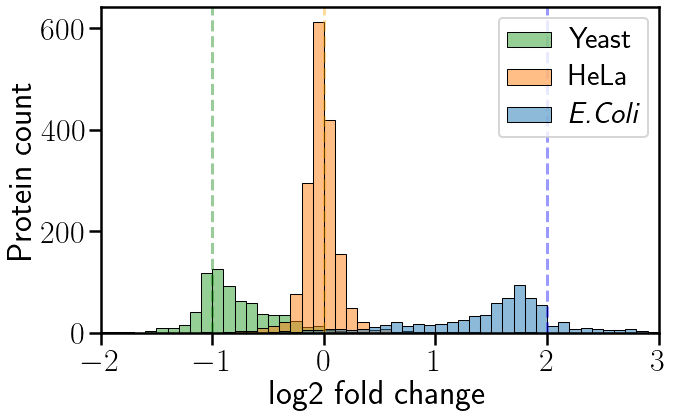
\includegraphics[width=0.4\linewidth]{../../result/report_plots_filtered/osw_triqler_intensity.png} & 
	    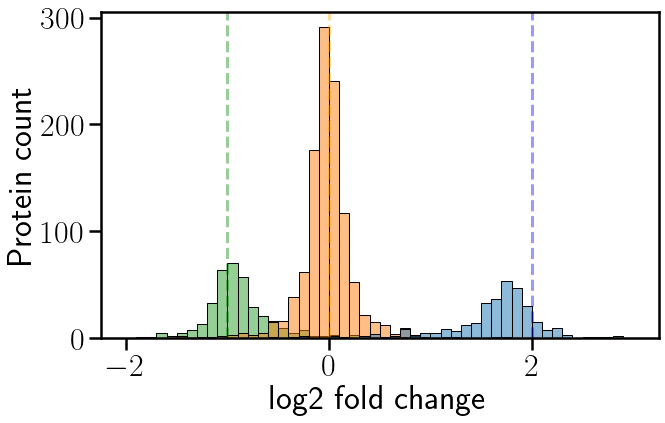
\includegraphics[width=0.4\linewidth]{../../result/report_plots_filtered/osw_top3_intensity.png} \\ 
        A & B \\ 
	    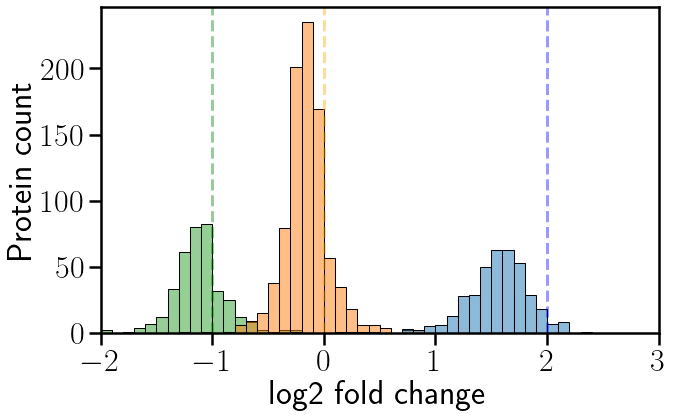
\includegraphics[width=0.4\linewidth]{../../result/report_plots_filtered/osw_msstats_intensity.png} & 
	    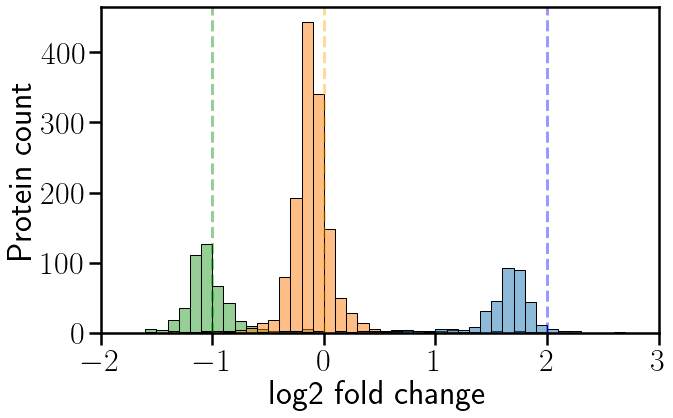
\includegraphics[width=0.4\linewidth]{../../result/report_plots_filtered/osw_msqrobsum_intensity.png} \\
        C & D 
    \end{tabular}
    \caption{{\bf Comparison of reported fold change distributions.} We used protein data from the ID spectral library pipeline and (A) Triqler, (B) Top3, (C) MSstats, and (D) MSqRob2. The dashed lines indicates the true log2-fold change ratio between a specie and HeLa samples. We noted that the empirical densities of the protein counts are less biased for Triqler and Top3 than MSstats and MSqRob2, the apex of their distribution were found closer to the true fold-change difference (see Supplementary Figure \ref{fig:fc_histogram_again} for reported fold change distributions for both ID and PS workflows). \label{fig:fc_histogram}}
\end{figure}

\subsubsection*{Comparison of ability to discriminate differentially from equivalently abundant proteins}

The LFQBench set contains varying concentrations of {\em E. Coli} and Yeast concentrations in a background of HeLa-cells. As the first test of performance, we hence compared the methods' ability to infer the differentially abundant {\em E. Coli} and Yeast protein as a function of the number of false positives from the HeLa-background, when varying the reported significance threshold from 0.0 to 0.1 with 0.001 increments (Figure \ref{fig:diff_vs_hela}). Overall, it seems like Triqler reports more differentially abundant protein for every non-differentially abundant protein for both the peptide abundances generated by the ID spectral library and PS spectral library pipelines. Surprisingly, Top3 performs has more true differentially abundant proteins for every false protein than MSstats. 

\begin{figure}[hbt]
    \centering
    \begin{tabular}{lclc} 
        A & 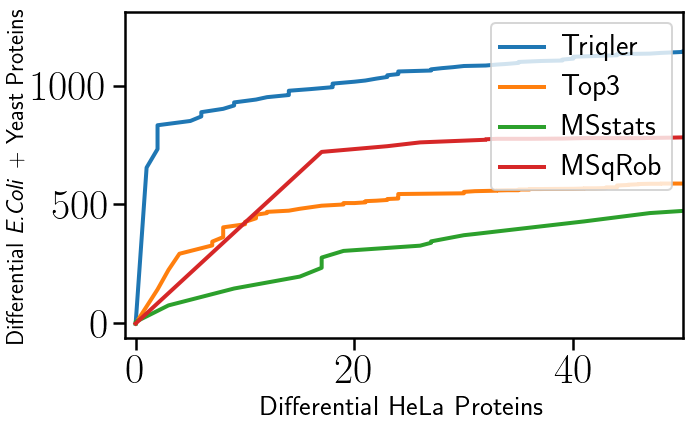
\includegraphics[width=0.45\linewidth]{../../result/report_plots_filtered/osw_de_human_vs_ecoli_and_yeast.png} & 
        B & 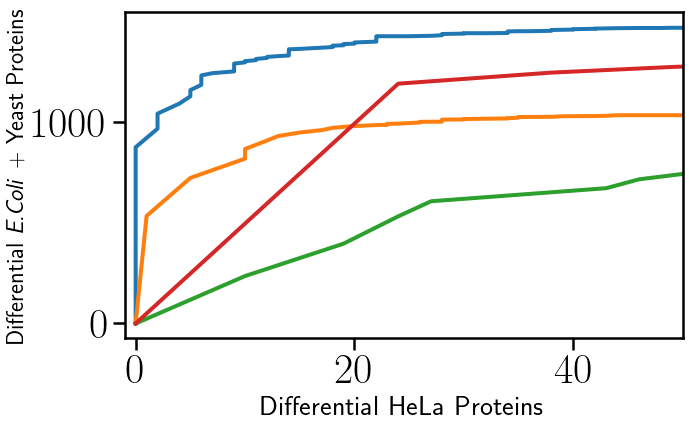
\includegraphics[width=0.45\linewidth]{../../result/report_plots_filtered/diann_de_human_vs_ecoli_and_yeast.png} \\ 

    \end{tabular} 
    \caption{{\bf Comparison of ability to differentiate proteins with differential abundance between conditions} We plotted the number of reported differentially abundant  {\em E. Coli} and Yeast proteins as a function of the number of proteins from the HeLa background when sorting according to significance for (A) DDA generated spectral libraries and (B) DIA-Umpire generated Pseudo spectra. For the test, we selected a fold-change threshold of 0.64 for Triqler, because it is the rounded average of the lower bound for fold-change computed by Triqler (Supplement Figure \ref{fig:ability_to_differentiate_differentially_abundant_specie_vs_hela} shows differential abundance for each specie). \label{fig:diff_vs_hela}}
\end{figure}

\subsubsection*{Comparison of statistical calibration}

We subsequently set out to test the statistical calibration of the different summarization methods. We hence investigated the relationship between the fraction of wrongly reported differential abundant proteins (i.e. the fraction of HeLa proteins among all reported differential abundant proteins), and each inference method's estimated false discovery rate (See Figure \ref{fig:frac_hela_vs_fdr}). We observe that Triqler, Top3, and MSqRob2 give estimates that are close to the true fold-change level than MSstats. This is somewhat surprising given that both MSstats and MSqRob2 are using the Benjamini-Hochberger corrections which are generally found more conservative than $q$~value estimates.

%We observed that Triqler and Top3 were reporting slightly more accurate estimates than MSstats and MSqRobSum. This is somewhat surprising given that both MSstats and MSqRobSum are using the Benjamini-Hochberger corrections which are generally found more conservative than $q$~value estimates.

\begin{figure}[hbt]
    \centering
    \begin{tabular}{cc} 
        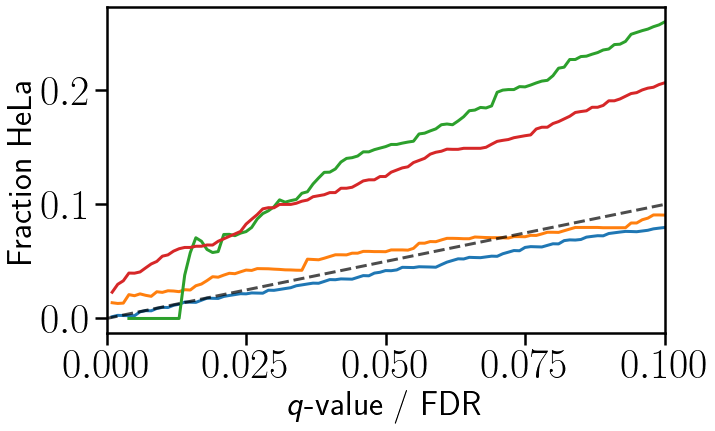
\includegraphics[width=0.5\linewidth]{../../result/report_plots_filtered/osw_FP_DE_all.png} & 
        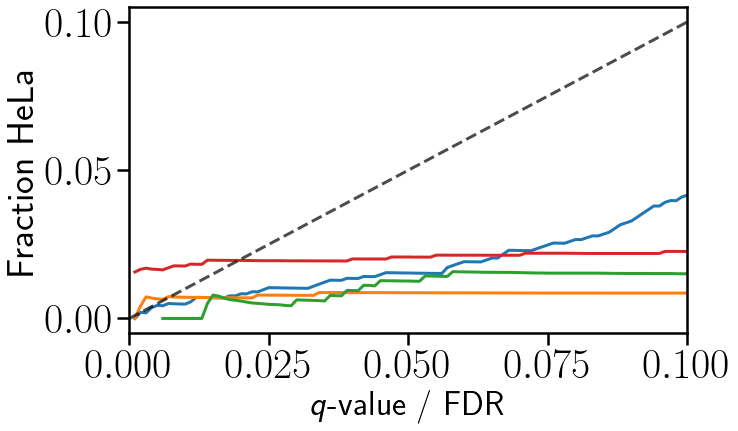
\includegraphics[width=0.5\linewidth]{../../result/report_plots_filtered/diann_FP_DE_all.png} \\
        A & B
    \end{tabular}
  \caption{{\bf Comparison of calibration of the compared summarization methods.} We plotted the fraction of reported differentially abundant HeLa proteins as a function of $q$~value treshhold for (A) ID spectral library pipeline and (B) PS spectral library pipeline. The multiple test correction is performed with $q$~value for Triqler and Top3, while Benjamini-Hochberger corrections was used for MSstats and MSqRob2. \label{fig:frac_hela_vs_fdr}}
\end{figure}

\subsubsection*{Differential abundance reported by the protein quantification tools.}


We also investigated the number of reported differential abundant proteins as reported by our four protein summarization methods. The results can be found in Supplementary Figure \ref{fig:da_methods_esimate}. We note that a larger number of reported differentially abundant proteins were reported by e.g. MSqRob2 than Triqler, however, this was likely due to the more lenient FDR estimates by MSqRob2.



\section*{Discussion}


Here we have shown that Triqler operates well for DIA data, despite originally intended for DDA data. We also find that Triqler outperforms other protein summarization methods on our engineered benchmark set, both in terms of sensitivity and accuracy in its error estimates. Triqler was also able to detect a significantly higher number of differentially abundant proteins at a more accurately reported false discovery rate, than the compared methods. 

The analytes in shotgun proteomics are peptides and not proteins or proteoforms. Nevertheless, most users of mass spectrometry use and will continue to find reasons to report findings on a protein level. It makes sense to put efforts into a better understanding of which protein inference tools to use at what occasion and how to summarize peptide abundances into protein relative concentration values.  Also, protein summarization gives lower variance than peptide-level analysis, and it reduces the number of hypotheses tested and reduced the number of missing values, which can have a major impact on the quality of the analysis \cite{plubell2021can}.   

One important remark is that the sequence database that we used for matching the spectra was filtered so that only one protein per peptide was kept, to control for any difference in protein inference strategies used by our compared protein summarization methods. There is currently no consensus on how to handle multiple proteoforms in bottom-up proteomics. Hence, we believe that protein inference strategies that can account for multiple proteoforms would greatly benefit the field by improving the quality of the quantitative analysis. 

We do see some differences in how DIA and DDA peptide-level abundance data appear. For instance, there are more missing values in DDA than DIA data. However, we find that qualitatively the types of data are similar, at least in the sense that Triqler's underlying assumption of missing values seems to be as valid for DDA and DIA data.

Lastly, we want to highlight the benefit and importance of datasets such as the one provided by Navarro et al. \cite{navarro2016multicenter}. These benchmarking datasets make it easy for the scientific community to investigate computational tools by providing a golden standard and significantly facilitating benchmark studies. 

\section*{Acknowledgements}


\section*{Funding}

This work was supported by grants from the Swedish Research Council (grant 2017-04030) 

\section*{Supporting information}

\bibliographystyle{plain}
%\bibliography{benchmark}
\bibliography{benchmark.bib}
\end{document}



